% (c) 2002 Matthew Boedicker <mboedick@mboedick.org> (original author) http://mboedick.org
% (c) 2003-2007 David J. Grant <davidgrant-at-gmail.com> http://www.davidgrant.ca
% (c) 2008 Nathaniel Johnston <nathaniel@nathanieljohnston.com> http://www.nathanieljohnston.com
% (c) 2011 Scott Clark <sc932@cornell.edu> http://cam.cornell.edu/~sc932
% (c) 2012 Arne Hassel <arne.hassel@gmail.com> http://megoth.wordpress.com/
%
%This work is licensed under the Creative Commons Attribution-Noncommercial-Share Alike 2.5 License. To view a copy of this license, visit http://creativecommons.org/licenses/by-nc-sa/2.5/ or send a letter to Creative Commons, 543 Howard Street, 5th Floor, San Francisco, California, 94105, USA.

\documentclass[letterpaper,11pt,norsk]{article}
\newlength{\outerbordwidth}
\pagestyle{empty}
\raggedbottom
\raggedright
\usepackage{babel}
\usepackage{float}
\usepackage[T1]{fontenc}
\usepackage{framed}
\usepackage{graphicx}
\usepackage[utf8]{inputenc}
\usepackage{tocloft}
\usepackage{url}
\usepackage[svgnames]{xcolor}
\usepackage{wrapfig}
\usepackage{tabularx}

%-----------------------------------------------------------

%Edit these values as you see fit

\setlength{\outerbordwidth}{3pt}  % Width of border outside of title bars
\definecolor{shadecolor}{gray}{0.75}  % Outer background color of title bars (0 = black, 1 = white)
\definecolor{shadecolorB}{gray}{0.93}  % Inner background color of title bars

%-----------------------------------------------------------

%Margin setup

\setlength{\evensidemargin}{-0.25in}
\setlength{\headheight}{-0.25in}
\setlength{\headsep}{0in}
\setlength{\oddsidemargin}{-0.25in}
\setlength{\paperheight}{11in}
\setlength{\paperwidth}{8.5in}
\setlength{\tabcolsep}{0in}
\setlength{\textheight}{9.75in}
\setlength{\textwidth}{7in}
\setlength{\topmargin}{-0.3in}
\setlength{\topskip}{0in}
\setlength{\voffset}{0.1in}

%-----------------------------------------------------------

%Custom commands

\newcommand{\resitem}[1]{\item #1 \vspace{-2pt}}

\newcommand{\resheading}[1]{\vspace{8pt}
  \parbox{\textwidth}{\setlength{\FrameSep}{\outerbordwidth}
    \begin{shaded}
\setlength{\fboxsep}{0pt}\framebox[\textwidth][l]{\setlength{\fboxsep}{4pt}\fcolorbox{shadecolorB}{shadecolorB}{\textbf{\sffamily{\mbox{~}\makebox[6.762in][l]{\large #1} \vphantom{p\^{E}}}}}}
    \end{shaded}
  }\vspace{-5pt}
}

\newcommand{\ressubheading}[4]{
\begin{tabularx}{6.5in}{l@{\cftdotfill{\cftsecdotsep}\extracolsep{\fill}}r}
		\textbf{#1} & #2 \\
		\textit{#3} & \textit{#4} \\
\end{tabularx}
\vspace{-6pt}
}

%-----------------------------------------------------------

\title{Curriculum Vitae}

\begin{document}

\begin{minipage}{\textwidth}
\begin{wrapfigure}{r}{0pt}
	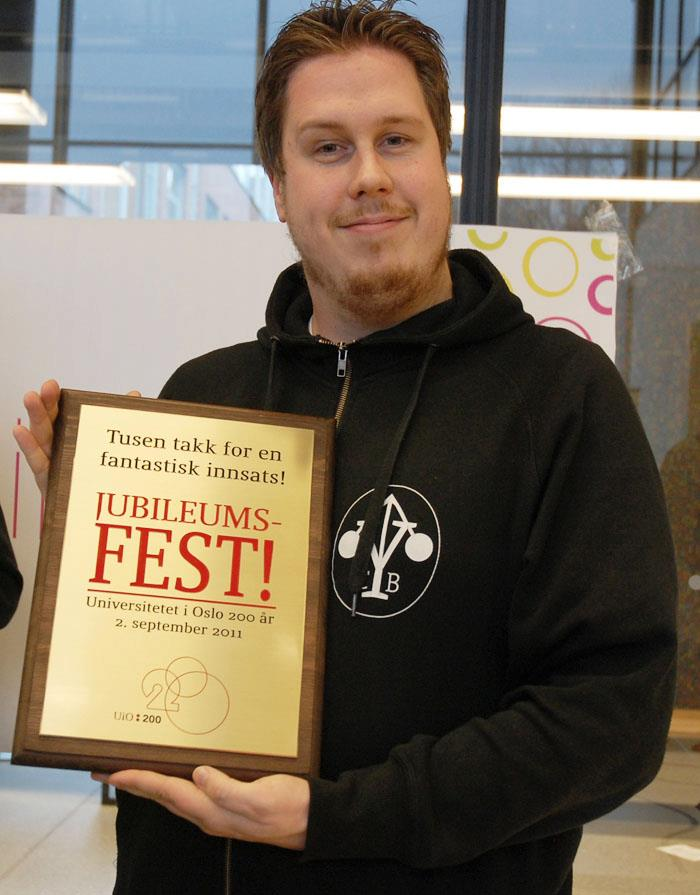
\includegraphics[height=45mm]{uio200.jpg}
\end{wrapfigure}

\textbf{\Large Curriculum Vitae for Arne Hassel}

\vspace{5mm}

\begin{tabular}{p{1in} l}
Adresse: & Rosenborggata 15c, 0356 Oslo\\
Telefon: & 416 94 086 \\
E-post: & \url{arne.hassel@gmail.com} \\
Født: & 5. desember 1984 \\
Sivilstatus: & Ugift \\
\end{tabular}

\vspace{5mm}

\begin{minipage}{5.5in}
Snart nyutdannet master i informatikk, med fokus på nettbaserte løsninger. Erfaren programmerer, løsningsorientert og setter meg raskt inn i ny teknologi og nye programmeringsspråk.
\end{minipage}

\end{minipage}

\resheading{Arbeidserfaring}

\begin{itemize}
\item
	\ressubheading{Senter for pasientmedvirkning og samhandlingsforskning}{Oslo}{Systemutvikler}{2008 - nåværende}
	\begin{itemize}
		\item Jobber for det meste med frontend (HTML, CSS og JavaScript), men har også jobbet en del med backend (.NET-plattformen)
	\end{itemize}
\item
	\ressubheading{Kiwi}{Risør \& Oslo}{Deltidsmedarbeider}{1999 - 2008}
\item
	\ressubheading{Senter for Helse \& Arbeid}{Oslo}{Personlig assistent}{2008}
\end{itemize}

\resheading{Utdanning}

\begin{itemize}
\item
	\ressubheading{Institutt for informatikk, Universitetet i Oslo}{Oslo}{Master i informatikk: programmering og nettverk (nåværende)}{2010 - 2012 (estimert)}
	\begin{itemize}
		\item Skriver masteroppgave om JavaScript og Semantisk Web, veiledere er Kjetil Kjernsmo og Martin Giese
		\item Programmert mye i Java og Eclipse
	\end{itemize}
\item
	\ressubheading{Institutt for informatikk, Universitetet i Oslo}{Oslo}{Profesjonsstudie, Distribuerte Systemer og Nettverk}{2007 - 2010}
\item
	\ressubheading{Universitetet for miljø og biovitenskap}{Ås}{Bachelor i økonomi og administrasjon}{2003 - 2007}
\item
	\ressubheading{Risør VGS}{Risør}{Allmenne fag}{2000 - 2003}
\end{itemize}

\resheading{Ferdigheter}

Se vedlagt kompetansediagram for ytterligere detaljer.

\begin{itemize}
\item {\bf Utvikling:} {\bf (Veldig god:)} CSS, HTML, JavaScript, LESS, Sass, SQL, {\bf (God:)} C\#, Java, PHP, Python, RDF, SPARQL, TTL, XML, XSLT, {\bf (Grei:)} Assembly, C
\item {\bf Rammeverk:} Compass, Django, .NET MVC 2 \& 3, Umbraco, Wordpress
\item {\bf Informatikk:} Databaser, semantiske teknologier, systemutvikling, algoritmer, datastrukturer, kvalitativ forskning, modellering, datamaskinarkitektur, \LaTeX, design patterns
\item {\bf Administrasjon:} Organisasjonsanalyse, SWOT-analyse, risikoanalyse
\item {\bf Økonomi:} Regnskap, budsjett, bilagsføring, samfunnsøkonomi
\item {\bf Språk:} Norsk (morsmål), engelsk (flytende)
\end{itemize}

\resheading{Utvalgte prosjekter}

\begin{itemize}
\item {\bf CommunicareTools:} Nettside med fokus på å presentere program-porteføljen til Senter for pasientmedvirkning og samhandlingsforskning. Utviklet i .NET med rammeverket Umbraco. \url{http://communicaretools.org/}
\item {\bf Zetti:} Et rapporthåndteringssystem som skal tas i bruk av driften til Cybernetisk Selskab. Utviklet i rammeverket Django og Compass. Under utvikling. \url{https://github.com/megoth/Zetti}
\end{itemize}

\resheading{Frivillig arbeid og tillitsverv}

\begin{itemize}
\item
	\ressubheading{Cybernetisk Selskab (CYB)}{Oslo}{Kasserer, økonomifunksjonær, fadderstyremedlem, vakt}{2009 - nåværende}
	\begin{itemize}
		\resitem{Satt i Hovedstyret som Kasserer høsten 2009 til og med våren 2011, nå med i økonomigruppen.}
		\resitem{Bygde opp det økonomiske systemet til å kunne ta i mot utfordringene i overgangen til CYB som instituttforening, driver av studentkjeller og nå største forening på Ifi.}
		\resitem{Var administrator/koordinator for Ifi-blekka 2011, en årlig utgivelse med informasjon til de nye studentene.}
	\end{itemize}
\item
	\ressubheading{Bursdagsfesten på Ole-Johan Dahls hus 2. september}{Oslo}{Festgeneral/Koordinator}{2011}
	\begin{itemize}
		\resitem{Planla, gjennomførte og avsluttet etterarbeidet tilknyttet Bursdagsfesten i anledning Universitetet i Oslos 200-års jubileumsfeiring.}
		\resitem{Samarbeidet med Ifi og UiO:200, jubileumsekretariatet, og lagde fest for nesten 5 000 mennesker.}
	\end{itemize}
\item
	\ressubheading{IAESTE}{Ås}{Dataansvarlig, leder, økonomiansvalig, nestleder}{2003 - 2007}
\item
	\ressubheading{UKA i Ås}{Ås}{Webansvarlig, Vertskap}{2004, 2006}
\end{itemize}

\resheading{Personlige detaljer}

\begin{itemize}
\item {\bf Hobbyer:} Lese, lære nye ting, bygge/lage nye ting (f.eks. i lego), brett-, kort- og rollespill
\item Har førerkort klasse B
\end{itemize}

\resheading{Referanser}

Jeg vil oversende en liste med mine referanser om dette skulle bli aktuelt.

\end{document}
